\section{Methods}


\subsection{Project Methodology}
When working in a project it is generally a good idea to work according to a predetermined project methodology model. This tends to make the work more effective and produce better quality. That is, more is produced during the same amount of time, the final product is more thought out, better teamwork etc.

Simply, if you have a plan at the start it is easier to stick to that plan and stay on the same path as intended, rather than shifting to another one. That is not to say that the plan cannot change, but if it does it does so controllably.

A historically good model has been the waterfall model. However, in the software industry this has changed lately with the agile methodology being more popular and has proven to be very effective.

\subsubsection{Agile}
Basically, the agile model says that rather than planning a workload for 6 months forward or so it is better to work in short iterations. These iterations should be between 1 - 4 weeks depending on the team.
Instead of trying to estimate the time it will take to complete an entire project, the team is given a finite time frame and tries to do as much as possible during that time. During this time, the team works very closely to the customer and project owner to make sure that they will get what they want and ask for.
For selecting items to work with for every sprint the team keeps a backlog of item it wishes to complete during the project. Every sprint these items (or stories) are picked out and included into the sprint and estimated in size. The stories themselves should be collected from customers, project owner, users and people connected to the product. This way, the team knows what the purpose is with developing a certain thing. If there is any doubt about a specific feature it should be easier to ask than to assume.

This is of course a simplified version of how the agile method works. 'Extreme Programming Pocket Guide' is a good book for anyone who wants to read more about agile methodology.

\cite{extremeProgramming}


\subsubsection{How we used the agile methodology}
\textbf{Sprints} \\
For our planned work we have decided to work in two week period sprints where we begin on a Tuesday and end on a Monday. At each start of a sprint we pick out stories to focus on for the coming two weeks and try to estimate how long each of them will take.
On weekdays we start with a quick discussion about yesterdays work and what we are planning to do today. This is for everyone to be up to speed about the other persons work.
At the end of the sprint everything is review and analysed so to do even better the next sprint by correcting possible faults.

\textbf{Story board} \\
For organizing our sprints we used a story board which contained an area for our backlog items and four rows for our stories during a sprint. The stories were broken into tasks which were placed on either one of the columns (Started, In Progress, Waiting, Completed).
Each story was estimated with a size which was a number in the fibonacci sequence. Each story was also divided into 5 parts (Started, Halfway done, Completed, Reviewed, Verified). These two numbers were multiplied and summed up with all the other stories to get how many points the sprints had. As we worked these points were subtracted and ultimately hit zero when we were done with everything. We plotted the progress on a chart as well for graphic. This is called a burndown.

\begin{figure}[hbtp]
\begin{center}
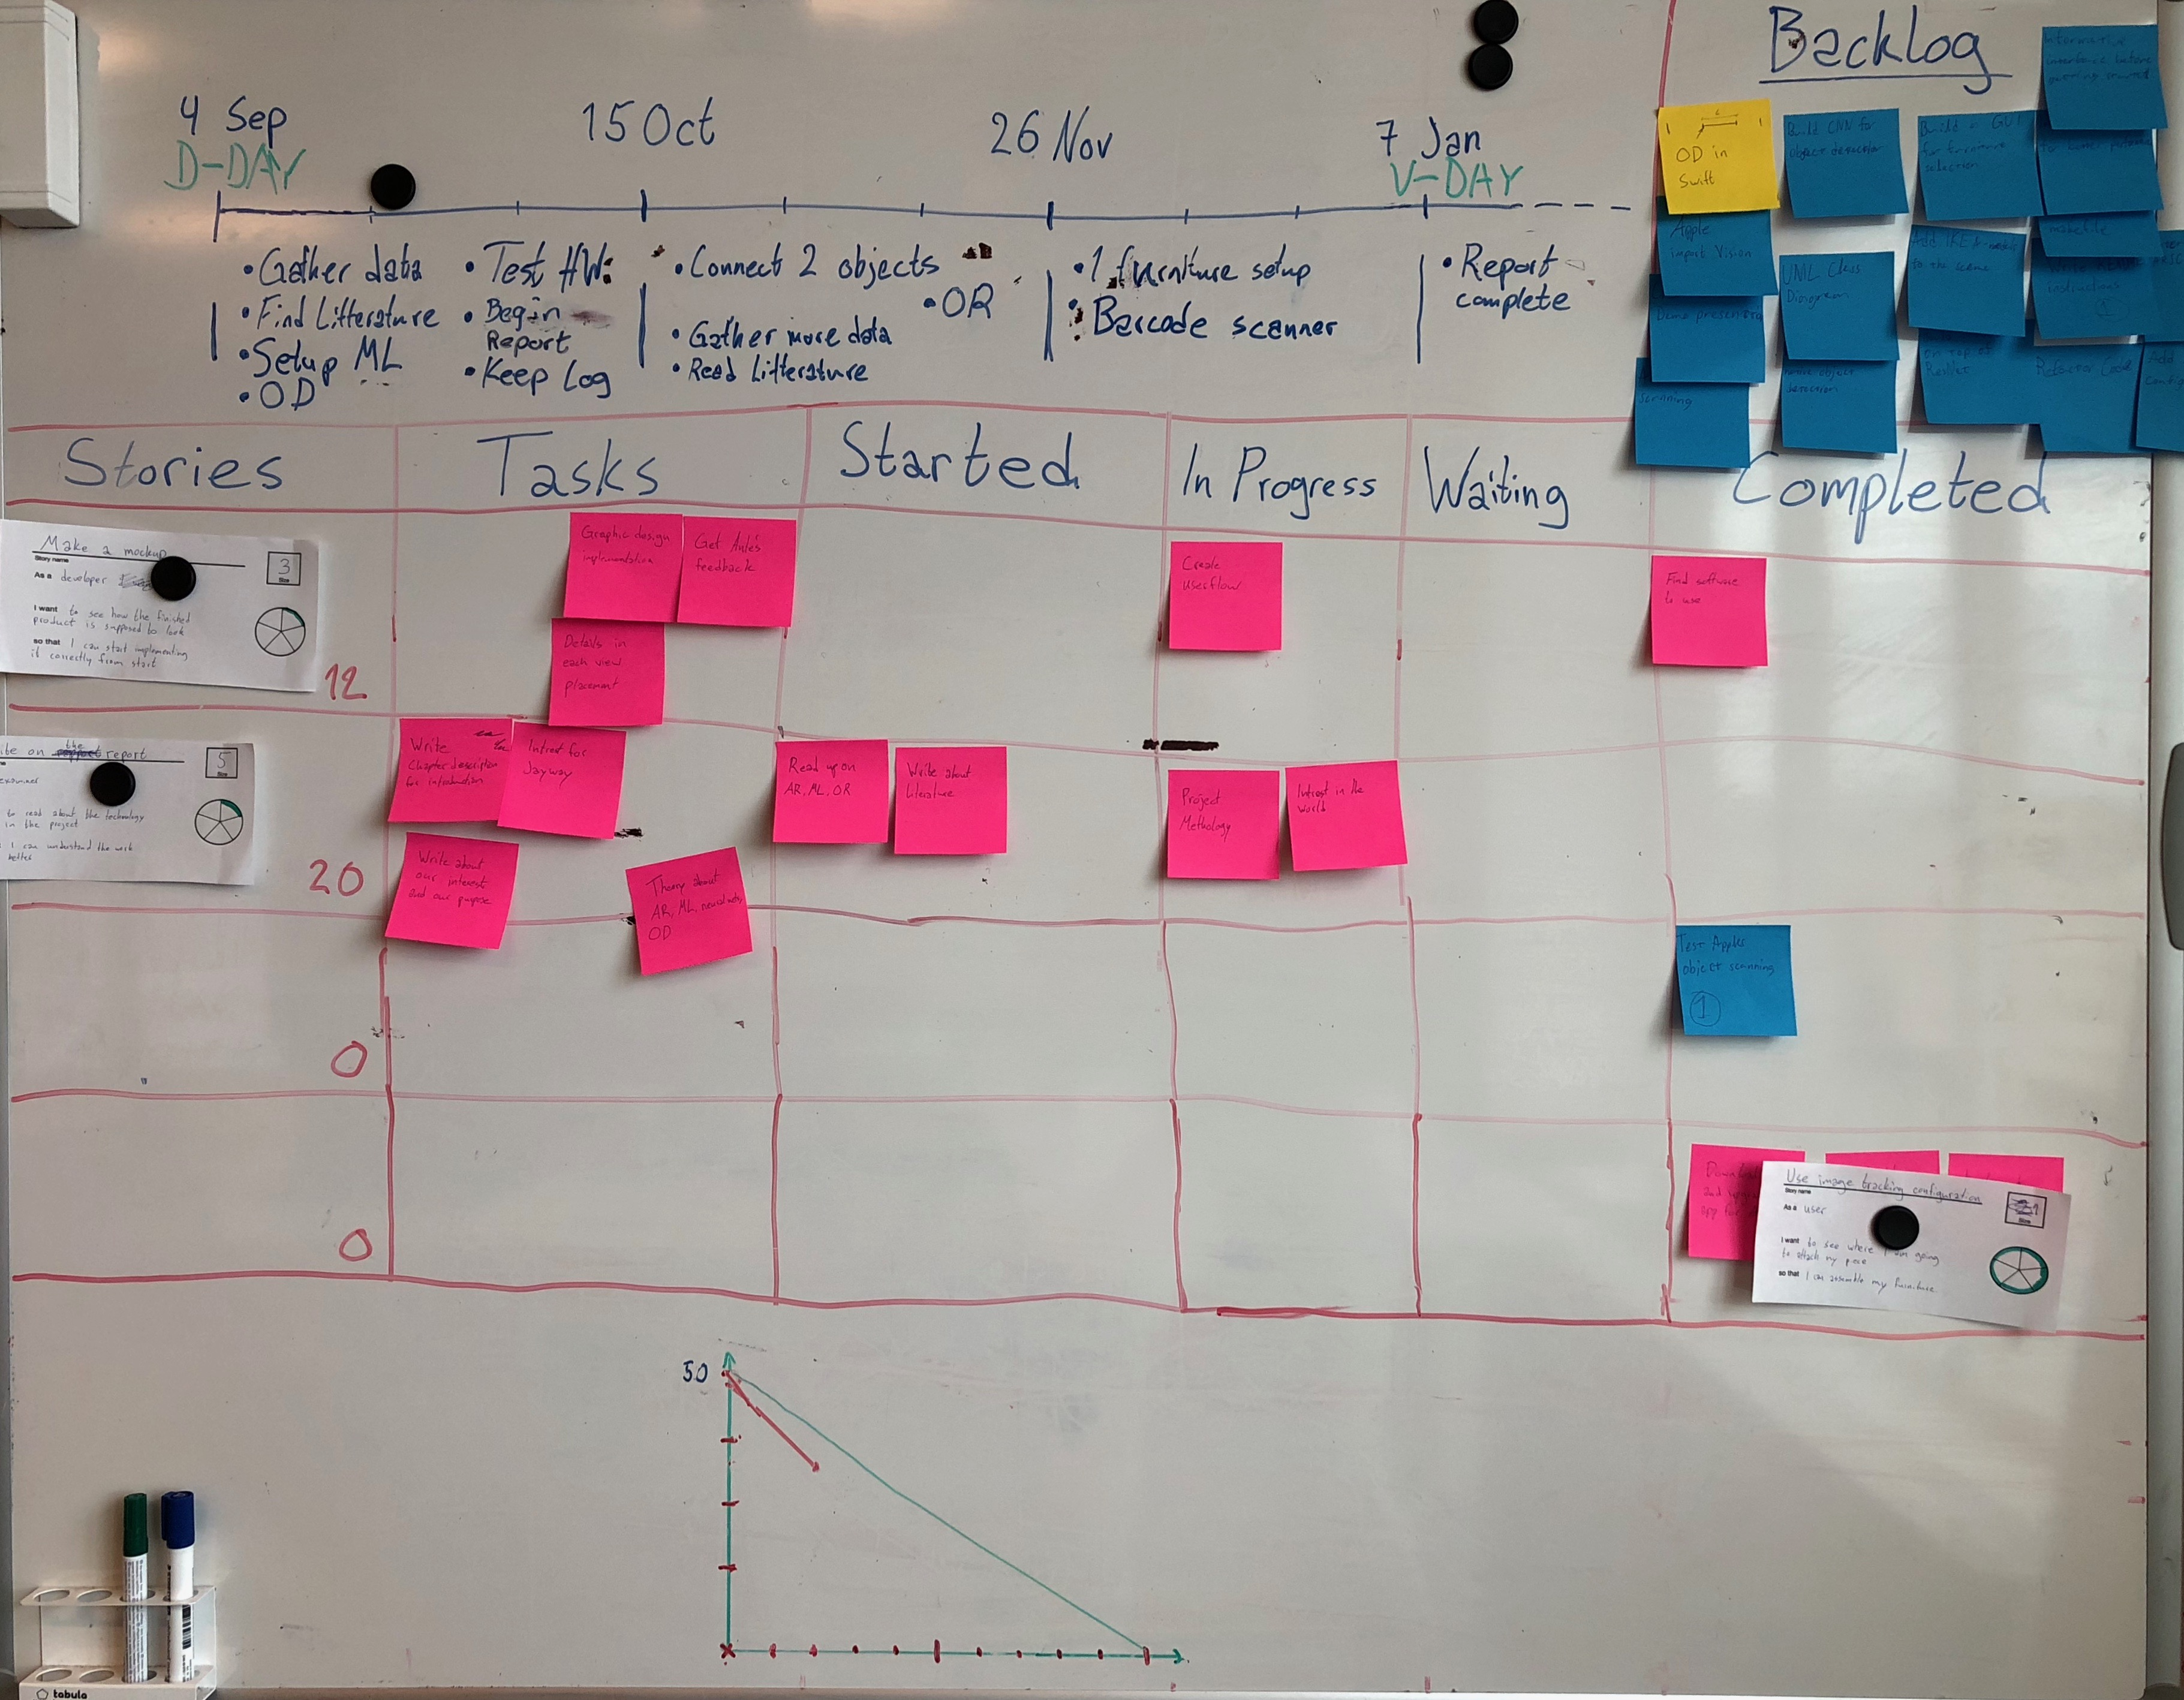
\includegraphics[width = 0.5\textwidth]{./Images/story_board.jpg} 
\caption{Story board used during the project}
\end{center}
\end{figure}


\textbf{Close relationship with project owner} \\
We worked very close to the project owner by sitting on desks right across him. Whenever we had a questing we could simply raise our head and ask it.

\subsection{Matlab prototype for Object Detection}
% Write about design decisions for the Matlab prototype and what it does. 
% Probably add some code as well.

\subsection{Collecting data}
When working with machine learning, big sets of data is often required for a good resulting model.
A problem with this is that it can be tricky to obtain such a large data set because it usually also requires
labels with that data to be manually input. These labels will be used by the neural net to, during training, check if
the predicted value is correct or not.

In this project the data is sets of images of different furniture parts. These images didn't exist anywhere online, so they had to be collected by taking lots of photos. The photos contained the part in different background and from different angles. The backgrounds were mostly of typical office surroundings, although there were exceptions (as will be explained shortly). All the photos were then resized to 256x256 pixels. The reason for choosing a square size is because when rotating them (this will be useful later on when augmenting data) the images will not have any black bars on the sides or be stretched.

For the first furniture Nolmyra, there were only 3 unique part (, excluding screws and similar parts). Therefore the model was trained to recognize 4 things; the different parts and an unknown object. The unknown label was because the object detection algorithm could detect other objects and it is then unwanted that those objects be mistaken for furniture parts. This could of course also be done by setting a threshold on the confidence value, i.e if the model give a confidence value under X it discards it as being an unknown object. The problem with this type is that it is much harder to distinguish parts from unknown objects. This is due to that the best model is the one that can give a close to 100\% confidence value on every prediction.

For this reason, photos of random objects were also added to the data set. Most of these photos were taken by ourselves, but some were also collected from the web. The images were placed in folders with a specific item which meant labelling them became much simpler. Just put all the images containing a certain part in the same folder.

Training a model usually requires hundreds of thousands or even millions of photos. That much data is hard to get and would take a lot of time to obtain Going around the office to snap that many photos is almost unthinkable.
However, there are other options.

\subsubsection{Augmenting data}
Instead of training on only original images, some images can be created from other images by for example rotating, flipping, changing brightness, saturation, contrast etc.  This will essentially be an image of the same object, but the data will look different, thus gives the model more relevant data to train on.
When doing this it is important to keep in mind that the augmented data should be relevant to real situations.
Creating data with only the blue color band when the real situations are only in daylight makes no sense.

Furthermore, images of objects of interest can be cut out and pasted into random environments to create even more data.
The idea of this is to try and make the model understand that the focus should be on the furniture part and the background environment is irrelevant. While doing this, even though the parts could be cut into totally random environments we tried to focus on pasting them into relevant spaces like office floors or carpets.
In our project, this gave a good results as it increased the test accuracy by 8%.

Doing this by hand can still be very time consuming, so automating this process as far as possible is recommended.

\subsection{Testing Object Scanning with ARKit2}
Apple's ARKit2 has a feature where it can detect scanned 3D objects. For scanning, they have developed an app that can be downloaded from their website. \cite{ARScanning}
After the scanning is complete the app lets you export the model to then include it in your ARKit2 project. Once in the project it is simply imported into the ARWorldTrackingConfiguration like shown below.

\lstinputlisting[language=swift,firstline=63,lastline=71]{../../Application/ObjectDetectionInAR/ObjectDetectionInAR/AssemblerViewController.swift}

\begin{figure}[hbtp]
\begin{center}
\includegraphics[width = 0.32\textwidth]{./Images/3dscanning1.png}
\includegraphics[width = 0.32\textwidth]{./Images/3dscanning2.png}
\includegraphics[width = 0.32\textwidth]{./Images/3dscanning3.png} 
\caption{3D Scanning using Apple's app. On the right, the bounding box is defined so that no reference points from other objects are included. In the middle, the object is scanned by aiming the camera around the object at all angles. On the right the created model is tested. In this case, the object is detected after 0.4 seconds.}
\end{center}
\end{figure}

Once imported into our project we were able to test the performance of recognizing and tracking three pieces of our furniture.
Sadly, this method came up short for our purpose. When testing live in our app the time for detection were much longer ( over 1 second ) which made tracking them difficult. The tracking wasn't smooth but rather choppy. Many times, the object wasn't detected at all. This was mainly due to our objects being a little big to fit the screen while being close with the camera but also that the object had a lot of empty space within its bounding box.

The detection worked best while being in the same environment, static with the same kind of lightning conditions, but fell short when the object was moving or being held. Therefore, since the user is going to hold the pieces by hand and moving them around, this method cannot be used for our purpose.

\subsection{Testing Object Tracking with Vision package}
Vision is a package from Apple which contains a lot of different methods for images and video. It contains still image analysis, image sequence analysis, object tracking, face detection etc.

On their website, Apple has a project that lets any user try out the object tracking on a video. When trying this on one of the furnitures we are going to assemble, the result was very promising. While the parts were laying on the floor and simultaneously moving the camera around, the objects were tracked fairly well. It was only when the camera was moved in such a way that made the pieces rotate in the picture that it started having a hard time tracking it.

For solving this, object detection can be performed in a reasonable time interval and be tracked until object detection is performed once again etc.

\cite{ObjectTracking}
The difference for this project and Apple's test project is that object tracking is going to be performed in real-time. This puts a limit on how many frames per second we can perform object tracking, since in a video playback you can just choose how fast you want to feed the new images. In real-time, the world doesn't stop moving.

After the system was implemented into our application different frame rates were tested. The optimal value was somewhere in-between 10-30 fps. If you went higher than that the application would become very choppy and eventually shut down.

Going lower than 10 fps the user will start to experience that the objects are hard to track in rapid movements.

For this application, however, the user is not going to encounter any scenarios where objects are flying around rapidly. Therefore we will settle for 20 fps as the optimal value for performance since any higher amounts don't really contribute to a better experience.

The following lines of code show how the object tracking was set up. One important thing to realize when setting this up is that the heavy calculations are run on a different thread than the main thread (in this case the work thread). 

That is why they can be executed in a while true loop. Later though, when drawing on the GUI wants to be made, they MUST be done on the main thread.

\lstinputlisting[language=swift,firstline=48,lastline=90]{../../Application/ObjectDetectionInAR/ObjectDetectionInAR/ObjectTracker.swift}


\subsection{Combining Object detection with Object Tracking}

\subsection{Design process of Machine Learning Model}
It was decided that a machine learning model for classification of different parts were to be designed using Keras [CITE]. Firstly, a lot of data would have to be gathered with which to train the network upon. Pictures of the different parts of the furniture was taken from several different angles and on various amounts of background floors. 
All images were scaled down to \imageSize to speed up the training process as well as remove possible unnecessary features [CITE]. To easily generate even more data, the images were rotated, had their brightness and sharpness altered. 
[INSERT IMAGE SET SHOWING DIFFERENT CONFIGURATIONS]
 
% Write about what design choices we made, from first iterations or planing, to our final model, add some code. 
\subsubsection{Deep Neural Networks}
% Write about that we chose Keras and that why made our model the way we did
In implementing the convolutional network several configurations were tried and further tested for accuracy in the developed application. What was tried was as follows:
[ADD IMAGES/TEST RESULTS]

\begin{itemize}
\item Changing amount of convolutional layers
\item Kernel sizes of the convolutional layers
\item Addition and removal of pooling layers
\item Stride sizes of the pooling layers
\item Layers in the fully connected part
\item Amount of nodes in the fully connected part
\item Addition of dropout to reduce chance of overfitting 
\end{itemize}

\subsubsection{Transfer Learning}
% Write about how we went about in order to insert Transfer Learning into the mix. 
After trial of designing the network from scratch, it was decided to try and make use of pre-trained networks and then retrain them for another purpose. Models trained on imageNet [CITE] were chosen since that source domain is similar to this target domain. The models with their respective weights were loaded, without their fully connected layer. The top layer's weights were then frozen at different stages, and new fully connected layers were added on top, and new classifiers were trained. 
Several different models were tried, including ResNet50[CITE], InceptionV3[CITE] and VGG19[CITE].
[ADD CODE]
[ADD IMAGES/TEST RESULTS]

\subsubsection{Turi Create}
%Write about the testing an implementation of Turi
Apple have developed their own toolkit for development of custom machine learning models called Turi Create \url{https://github.com/apple/turicreate}. This was created to help developers to easily implement their own ideas into an app. It includes methods for image classification, object detection etc.. 

In this project, the Object Detection method included in Turi Create was tested. First, one has to create ground truth data for every image that was trained and tested on. This was done using Simple Image Annotator \url{https://github.com/sgp715/simple_image_annotator}, where one has to draw bounding boxes for the objects in the images and label them; the data output is in the \textit{.csv} format.  Turi Create uses a different format for annotations called \textit{.sframe}, however, they provide a simple Python script which automatically does the conversion. 

Turi then trains a model using a re-implementation of the TinyYOLO netwok. It also utilizes transfer learning by starting with an image classifier that has been trained on the imageNet dataset and the does \textit{end-to-end finetuning} do change the network to a \textit{one-stage detector}.

After training and evaluating that the model lives up to a standard worth including in this project, it was converted to the \textit{.mlmodel} format usable by CoreML in the application. However, due to current technical bugs in Turi Create the model does not yield correct bounding boxes while running in the application, thus the decision was made to scrap the use of this toolkit.

[iNCLUDE IMAGES FROM TESTING BOTH IN TURI AND FROM TESTING IN APP] 

\subsection{AR implementation in ARKit}

\newpage

\begin{center}
\textbf{Log book}
\end{center}

\textbf{2018-09-18}
When training the object recognition net, they where trained on only the red channel and although it technically worked by inputting an RGB image later on, it obviously gave us completely bogus results.